\chapter{Pruebas}
\label{pruebas}

Una vez creada la primera versión de twinX, el siguiente paso es evaluar el trabajo llevado a cabo. Para ello, nos guiaremos por una serie de pruebas de las que poder obtener retroalimentación sobre si el software cumple las expectativas o si por lo contrario necesita mejoras, en contraposición de lo planeado en el desarrollo del proyecto.

\section{Pruebas de usabilidad}

En primer lugar, vamos a desarrollar cómo fueron las pruebas de usabilidad de twinX. La utilidad de estas pruebas está en conocer cuán buena es la disposición de los elementos del sitio y si su funcionamiento es adecuado, mediante la evaluación de la interacción de los usuarios con twinX.

Para llevarlas a cabo, se solicitó a dos usuarios que trabajan en la ORI-FyL que usaran la aplicación. Más concretamente, se les instó a que realizaran una serie de tareas en la web tras tener acceso a ella, sin darles ningún indicio de dónde tenían que acudir para llevar a cabo la tarea encomendada. De este modo, comprobamos si es o no sencillo utilizar twinX y qué mejoras se pueden hacer basadas en la interacción del usuario con la plataforma. Por ejemplo, si a la hora de realizar una acción que se solicite, todos los usuarios llevados a examen realizan la misma acción de forma errónea, entonces podemos afirmar que la aproximación propuesta tras el desarrollo no es válida, pues no funciona como se espera, y hace a los usuarios perder tiempo y la concentración con respecto a la consecución de sus objetivos.

Las sesiones de prueba se llevaron a cabo a través de Google Meet \cite{googlemeet} y se pidió permiso a los asistentes para grabar la sesión, de modo que pudiera ser examinada \textit{a posteriori}. A los usuarios se les solicitó que no entraran juntos a la sala de reunión para no conocer de partida el funcionamiento de la web antes de enfrentarse a las pruebas. Antes de ponernos manos a la obra, se les dio una pequeña introducción con unas pautas sencillas \cite{krug} y que hacían la sesión más fructífera y natural tanto para el evaluador como para los evaluados. Entre ellas, destacan las siguientes:

\begin{itemize}
	\item \textbf{Pensar en voz alta:} cualquier apreciación es buena. Pensamientos como «imagino que si pulso este botón iré a esta otra parte...» o «vaya, creía que iba a encontrar otra cosa» ayudan a la mejora y a reconsiderar las decisiones tomadas.
	\item \textbf{El usuario sometido a pruebas nunca se equivoca:} en todo caso, el fallo lo comete el desarrollador por haber pensado que algo podía ser buena idea pero finalmente termina confundiendo al usuario.
	\item \textbf{No complicarse la vida, actuar como se crea:} de lo contrario, el portal sería difícil de comprender, lo que no es beneficioso en absoluto.	
\end{itemize}

En twinX ya había cierta información introducida, como algunos estudiantes, países, universidades, tipos de expedientes y sus fases, y convenios, sobre todo, ya que albergan mucha información y tampoco sería apropiado excederse en tiempo haciendo pruebas con el usuario.

Las tareas que se solicitaron llevar a cabo a ambos usuarios fueron las siguientes:

\begin{enumerate}
	\item \textbf{Crear un acuerdo de estudios a uno de los estudiantes almacenados:} para ello hay que ir al apartado de acuerdos de estudios, situado en el menú de la izquierda en la sección de «gestión», que es la que se abre por defecto al entrar a twinX. Una vez allí, hay que pulsar el botón verde en la esquina superior derecha de la tabla y rellenar el formulario que se muestra a continuación.
	\item \textbf{Comprobar que el convenio tiene asociado el nuevo acuerdo de estudios:} de nuevo en el menú de la izquierda, hay que ir al apartado de convenios y buscar el convenio para el que se ha creado el acuerdo de estudios. Dentro de la vista, hay que desplegar la parte llamada «acuerdos de estudios» y ver que, efectivamente, figura el acuerdo de estudios que se acaba de crear asociado al estudiante correspondiente.
	\item \textbf{Crear un expediente para el acuerdo creado:} en el apartado de expedientes, hay que seleccionar la opción de «nuevo expediente». En el formulario, rellenar con el acuerdo de estudios que se ha creado en la primera tarea y seleccionar el tipo de expediente.
	\item \textbf{Introducir una primera fase para el expediente que se acaba de crear:} una vez creado, twinX redirige al usuario a la vista de expediente con sus fases en una tabla que se encontrará vacía de forma preliminar. A continuación, el usuario tiene que pulsar el botón de «nueva fase» y guardar los cambios. Una vez se muestra la lista con las dos fases asociadas al expediente, habría que pulsar en el botón con la flecha para procesar la fase. Se abrirá un cuadro de diálogo que hay que aceptar para completar el proceso.
	\item \textbf{Crear una nueva fase final para el tipo de expediente con el que se está trabajando:} en esta ocasión, la tarea requiere salir de la sección de «gestión» y dirigirse al panel de control. Allí, seleccionar el menú «expedientes», después de lo cual se desplegará un menú con otras dos opciones. Hay que escoger la de «fases de expedientes» y crear ahí una nueva fase para el tipo de expediente que se ha abierto al estudiante en la tercera tarea, marcando la opción de «fase final».
	\item \textbf{Cambiar el expediente a la fase recién creada:} volver a «gestión», en el menú del expediente con el que estamos trabajando. De nuevo, volver a asociar una nueva fase (la creada).
	\item \textbf{Consultar los acuerdos de estudios que tiene un tutor:} tan solo habría que ir al menú de tutores y buscar el único tutor que hay en la plataforma creado y al que se le puede asociar un acuerdo de estudios. Allí, hay que seleccionar la única acción disponible, que es un botón con un pergamino (el mismo icono que tienen los acuerdos de estudios) para acceder a una vista donde se muestran todos los acuerdos que tutoriza dicha persona. 
\end{enumerate}
%«Modificación del acuerdo OUT» (usuario A) y «Nominación IN» (usuario B)


\subsection{Sesión de pruebas del usuario A}

Para el usuario A, el desarrollo de las tareas (en el mismo orden que las hemos presentado) ha sido el siguiente:

\begin{enumerate}
	\item Primeramente se dirigió al menú de estudiantes. Al ver en la tabla que para cada estudiante tenía dos posibles acciones, reconoció que una era para ver los detalles del estudiante (botón del ojo) y el otro (universidad, para acceder a su convenio), no lo reconocía. Por tanto, puso el ratón encima y tal y como estaba previsto, apareció la ayuda textual que señalaba que era un botón para ir al convenio del estudiante. Entonces, cambió de estrategia y fue al menú de acuerdos de estudios, donde finalmente encontró la forma de desarrollar la tarea solicitada.
	\item A pesar de haber un botón en el acuerdo de estudios como acceso directo al convenio, que es donde se tenía que dirigir, fue al listado de todos los convenios y buscó el convenio para el cual se había creado el acuerdo. Al entrar en la vista del convenio, no reconoció dónde estaban sus acuerdos asociados; es decir, no supo interpretar que cada una de las categorías era desplegable y que al pulsarlas se vería nueva información tal y como se pensaba en el desarrollo que sugeriría la flecha hacia abajo de desplegable. Entonces, volvió al menú de acuerdos, donde anunciaba que efectivamente el acuerdo se había creado porque aparecía ahí. Sin embargo, se volvió a pedir al usuario que lo visualizara desde la vista del convenio. Volvió a la misma vista de antes y se paró a leer los enunciados de los desplegables. Daba la sensación de que en su primera visita, en el primerísimo vistazo, pensaba que las distintas secciones era más información del convenio. Al leer el de «acuerdos de estudios», efectivamente pulsó y comprobó lo que se le había solicitado.
	\item Para la creación del expediente, el usuario fue al menú del acuerdo creado, pensando que al entrar a verlo habría un botón para crear un expediente. Pero no encontró nada. Al percatarse de ello, fue al menú de expedientes, donde sí pudo ver de nuevo el botón verde que le permitía crear una nueva entrada.
	\item Al situarse justo debajo del acuerdo el botón que le permitía crear una nueva fase, el usuario A lo encontró rápidamente y pudo crear la fase en cuestión de segundos. Para procesar la fase, volvió a analizar los botones representando las tres acciones acompañadas de los iconos del lápiz, la papelera y la flecha. Supuso que éste último era para lo que buscaba y la ayuda de texto al posicionar el cursor encima se lo confirmó, pero también optó por hacerlo editando el registro y marcando la casilla «procesada» en el formulario de edición.
	\item Para explicar esta tarea, se pidió que volviera a crear una fase al expediente, y comprobó que efectivamente había solo una fase. Entonces, una vez comprendió el problema, fue muy directo al panel de control. Allí se desorientó un poco y se puso a observar todos los detalles. Entonces, tras recordarle la tarea, y tras haber leído todas las opciones del menú en la primera pasada, desplegó el menú correspondiente y accedió a la parte de «fases de expedientes». Una vez allí, creó la fase sin problema.
	\item Casi sin pedírselo y prácticamente curioseando, volvió a «gestión», a expedientes, creó la fase, la dejó sin procesar. Libremente se dirigió al dashboard, comprobó que había una fase sin procesar. Volvió atrás, procesó la fase y comprobó una vez más que en el dashboard no quedaba ninguna fase pendiente.
	\item Accedió al menú de tutores sin problema y pulsó sobre la única acción que había en el registro del tutor, completando la tarea y terminando, así, las pruebas.
\end{enumerate}

Este usuario se tomó muy en serio, afortunadamente, el «pensar en voz alta», lo que fue bastante positivo para poder comprender cómo pensaba. Hizo muchos comentarios como «me iría aquí...» o «supongo que si hago clic aquí, aparecerá esto otro...». También le llamó la atención el dashboard, y lo consultó por cuenta propia para ver que efectivamente, tras procesar un expediente, el registro desaparecía del resumen de «expedientes sin procesar», lo cual es bastante positivo. Además destaca la gran confianza que adquirió en la penúltima tarea, pues parecía haber estado trabajando con la aplicación anteriormente y denotaba haber comprendido muy bien la disposición de los elementos en la misma.

\subsection{Sesión de pruebas del usuario B}


Siguiendo el mismo orden, el otro usuario realizó también sus tareas como describimos:

\begin{enumerate}
	\item De nuevo, este usuario fue al menú de estudiantes. Se situó en el estudiante que se le indicó y cargó su vista. Una vez allí, trató de editar sus datos. Estuvo mirando otras características y probando otras funciones, como la de enviar mail al estudiante. Una vez volvió, sí fue directamente al menú de acuerdo de estudios y creó el convenio correctamente.
	\item Al haber estado en el paso anterior ojeando cómo son las vistas de los convenios, no le fue nada difícil encontrar el camino hacia el objetivo. Adicionalmente, reconoció el significado de la columna «nominados totales» del menú de convenios, algo muy positivo, ya que supone un gran cambio en cuanto a la visualización del mismo dato existente en TWINS (los primeros cuadros de colores en la figura \ref{fig:vistaConvenios}).
	\item Esta tarea fue también muy rápida, pues hizo click directamente en el menú de expedientes y en el botón verde de «nuevo expediente».
	\item De nuevo, al aparecer el botón de «nueva fase» en la vista tras crear el expediente, supo seguidamente crearla. Para procesarla, estuvo dudando sobre el botón de edición, el del lápiz --sobre el que posó el ratón--,  y el de «procesar fase». Finalmente, pulsó este último y aceptó el diálogo que concluía con esta tarea.
	\item Para esta tarea, tras la explicación, estuvo dudando bastante sobre cómo hacerlo: intentó escribir en el campo de búsqueda de la fase, fue atrás, hacia el menú de la vista de las fases del expediente, trató de editar el expediente del estudiante, pero ahí no estaba la opción. Finalmente, se le dieron indicaciones para que prestara atención a la cabecera de la web, la cual no había tomado como tal y desconocía que se albergaban más opciones ahí. Tras volver a curiosear entre las nuevas posibilidades que había descubierto, se dirigió al panel de control. Una vez allí, al menú de fases de expedientes, pero comenzó a introducir la nueva información en los campos destinados a la búsqueda. Sin la ayuda de nadie, se dio cuenta, y volvió a ejecutar las acciones desde el principio (en lugar de borrar su búsqueda o darle al botón de «nuevo expediente»). De nuevo en el menú correspondiente, ya sí supo crear lo que se le requirió.
	\item Al igual que el usuario A, recordó los pasos que había que hacer para volver a cambiar el expediente de fase. No obstante, tuvo la iniciativa de intentar llegar al mismo sitio siguiendo otro camino, pero finalmente tuvo que reproducir los pasos anteriores. Hizo clic en procesar la fase que ya habíamos procesado anteriormente, pero se dio cuenta a tiempo de que justo es lo que había hecho antes y no lo que se le solicitaba ahora, y canceló el diálogo a tiempo. Después, cambió el expediente a la fase recién creada.
	\item Esta tarea también fue muy sencilla para el usuario B y pudo completarla en cuestión de segundos.
	
\end{enumerate}

Del usuario B destacamos la gran curiosidad que tenía por descubrir cosas por su cuenta y ver los cambios que presentaba twinX. Algo de lo más positivo al hacer pruebas, fue su actitud «caótica» a la hora de ejecutar las acciones sin pensar, pues se dejaba llevar por su instinto y permitía ver las cosas que realmente estaban bien y las que no tanto. También comparaba algunas pequeñas carencias que no tenía TWINS respecto de twinX provenientes del uso diario de la aplicación, como un aumento de los accesos directos para ir fácilmente de una entidad a otra (por ejemplo, de la vista de estudiante a sus expedientes).

\subsection{Encuestas SUS}

Al final de la sesión, se ofreció a los individuos una encuesta SUS para que la cumplimentaran y así poder obtener más información de su experiencia. La rellenaron mediante los Formularios de Google \cite{googleforms}, y sus respuestas fueron los de las tablas \ref{tab:sus1} y \ref{tab:sus2}

\subsubsection*{Resultado 1}

\begin{table}[H]
	\begin{center}
		\begin{adjustbox}{width=\textwidth}
			\begin{tabular}{ | c | c | c | c | c | c | } 
				\hline
				\textbf{Pregunta} & 1 & 2 & 3 & 4 & 5 \\
				\hline
				Creo que utilizaría twinX con frecuencia &  &  &  &  & X \\
				\hline
				Encuentro twinX innecesariamente complejo &  X &  &  &  &  \\
				\hline
				Pienso que twinX es sencillo de usar &  &  &  &  & X \\
				\hline
				Considero que necesitaría la ayuda de una persona especializada para usar el sistema & X &  &  &  &  \\
				\hline
				Encuentro las funcionalidades de twinX bien integradas &  &  &  & X &  \\
				\hline
				Veo que hay mucha inconsistencia en el sistema & X &  &  &  &  \\
				\hline
				Imagino que la gente aprenderá rápido a usar twinX &  &  &  &  & X \\
				\hline
				Creo que twinX es demasiado engorroso para mí & X &  &  &  &  \\
				\hline
				Me siento muy seguro/a de mí mismo/a utilizando twinX &  &  &  &  & X \\
				\hline
				Necesitaría aprender bastantes cosas antes de comenzar a usar twinX & X &  &  &  &  \\
				\hline
			\end{tabular}
		\end{adjustbox}
		\caption{Resultado de la encuesta SUS 1}
		\label{tab:sus1}
	\end{center}
\end{table}

\subsubsection*{Resultado 2}

\begin{table}[H]
	\begin{center}
		\begin{adjustbox}{width=\textwidth}
			\begin{tabular}{ | c | c | c | c | c | c | } 
				\hline
				\textbf{Pregunta} & 1 & 2 & 3 & 4 & 5 \\
				\hline
				Creo que utilizaría twinX con frecuencia &  &  &  &  & X \\
				\hline
				Encuentro twinX innecesariamente complejo &  X &  &  &  &  \\
				\hline
				Pienso que twinX es sencillo de usar &  &  &  &  & X \\
				\hline
				Considero que necesitaría la ayuda de una persona especializada para usar el sistema &  &  &  &  & X \\
				\hline
				Encuentro las funcionalidades de twinX bien integradas &  &  &  &  & X \\
				\hline
				Veo que hay mucha inconsistencia en el sistema & X &  &  &  &  \\
				\hline
				Imagino que la gente aprenderá rápido a usar twinX &  &  &  &  & X \\
				\hline
				Creo que twinX es demasiado engorroso para mí & X &  &  &  &  \\
				\hline
				Me siento muy seguro/a de mí mismo/a utilizando twinX &  &  &  & X &  \\
				\hline
				Necesitaría aprender bastantes cosas antes de comenzar a usar twinX &  & X &  &  &  \\
				\hline
			\end{tabular}
		\end{adjustbox}
		\caption{Resultado de la encuesta SUS 2}
		\label{tab:sus2}
	\end{center}
\end{table}

\subsection{Conclusiones de las pruebas de usabilidad}

La respuesta de los usuarios ante las tareas solicitadas para ser llevadas a cabo ha sido muy positiva, si bien hay que tener en cuenta las confusiones que han tenido momentáneamente, que en ocasiones acompañaban a la personalidad del usuario y su forma de interaccionar con una interfaz completamente nueva.

Gracias a las pruebas realizadas, se puede comenzar desde ya a mejorar twinX incluso en su primera versión, sin planificar nuevas historias de usuario. Estas aportaciones son posibles debido a que los usuarios con los que se han hecho las pruebas trabajan en la oficina, lo que nos lleva a pensar que, como es lógico, el probar twinX en su misma atmósfera de trabajo tendría como resultado su exponencial potenciación a base de la diaria observación de la interacción con el actual TWINS, teniendo aún más información de aspectos que mejorar, a pesar del cambio que supone la nueva plataforma.

Sobre las encuestas, hay que clarificar que se han dispuesto en un orden aleatorio y que no se conoce cuál pertenece al usuario A y cuál al B. Para analizar mejor su resultado, vamos a dividir las preguntas en dos grupos: positivas y negativas (tabla \ref{tab:resultadossus}). Las primeras serán aquellas para las que cuantos más puntos se obtenga, más positiva será la valoración y viceversa. 

\begin{table}[H]
	\begin{center}
		\begin{adjustbox}{width=\textwidth}
			\begin{tabular}{ | c | c | c | } 
				\hline
				\textbf{Categoría} & \textbf{Preguntas} & \textbf{Puntuación} \\
				\hline
				\multirow{5}{*}{Positivas} &
				Creo que utilizaría twinX con frecuencia  & \multirow{5}{*}{48/50} \\
				\cline{2-2}
				& Encuentro las funcionalidades de twinX bien integradas & \\
				\cline{2-2}
				& Pienso que twinX es sencillo de usar &  \\
				\cline{2-2}
				& Imagino que la gente aprenderá rápido a usar twinX & \\
				\cline{2-2}
				& Me siento muy seguro/a de mí mismo/a utilizando twinX &  \\
				\hline
				\multirow{5}{*}{Negativas}& Encuentro twinX innecesariamente complejo & \multirow{5}{*}{15/50} \\
				\cline{2-2}
				& Considero que necesitaría la ayuda de una persona especializada para usar el sistema & \\
				\cline{2-2}
				& Veo que hay mucha inconsistencia en el sistema & \\
				\cline{2-2}
				& Creo que twinX es demasiado engorroso para mí & \\
				\cline{2-2}
				& Necesitaría aprender bastantes cosas antes de comenzar a usar twinX &\\
				\hline
			\end{tabular}
		\end{adjustbox}
		\caption{Resultado de las encuestas SUS}
		\label{tab:resultadossus}
	\end{center}
\end{table}

Es observable que en los aspectos positivos se roza el máximo de 50 puntos, mientras que por lo bajo, también se acerca a 10, siendo ésta la puntuación mínima, por lo que podemos apreciar que los resultados han sido buenos.

Si quisiéramos obtener un resultado sobre 100 acerca de cuán bien les ha parecido twinX a los usuarios, podríamos seguir las directrices que se indican en \cite{susscore}. Hemos de restar un punto a las preguntas impares y sustraer a 5 el valor de las pares. El resultado de sumar los nuevos valores y multiplicar por 2.5 daría, en cada encuesta, el resultado sobre 100. En el primer caso, habríamos obtenido una puntuación de 97.5 puntos y, en el segundo de 85 puntos. Sobre esta última, en un intento de comprender la respuesta a la pregunta «considero que necesitaría la ayuda de una persona especializada para usar el sistema», contestada con 5 (totalmente de acuerdo), podría ser por la necesidad de comprender el funcionamiento de la oficina, ya que basándonos en el resto de sus respuestas, parece haber tenido una buena experiencia tras las pruebas; es más, la puntuación que obtenemos es de 85/100, cuando 68 sería la media según la fuente que citamos.

En resumen, parece que el trabajo hecho con twinX no se distancia mucho de la línea en que desarrollan su trabajo en la ORI-FyL, por lo que podemos entender que se están consiguiendo los objetivos propuestos para el proyecto.

\section{Pruebas de accesibilidad}

Tal y como comentamos en la sección \ref{subsec:accesibilidad}, no todo el mundo tiene las mismas necesidades, y es hora de conocer si nuestro sitio web reúne una serie de condiciones mínimas para la visualización por personas con alguna discapacidad.

Por lo general, los resultados arrojados no son malos. La puntuación más baja que se ha obtenido ha sido la de 79/100 (figura \ref{fig:testaccesibilidad}), específicamente en las vistas de menú, donde los botones de la tabla (columna «acciones») tienen un icono visual y no un texto. Este problema se podría resolver fácilmente ofreciendo un texto alternativo para cada botón, de modo que un asistente de voz pueda leer la web, a pesar de tener elementos gráficos.


\begin{figure}
	\centering
	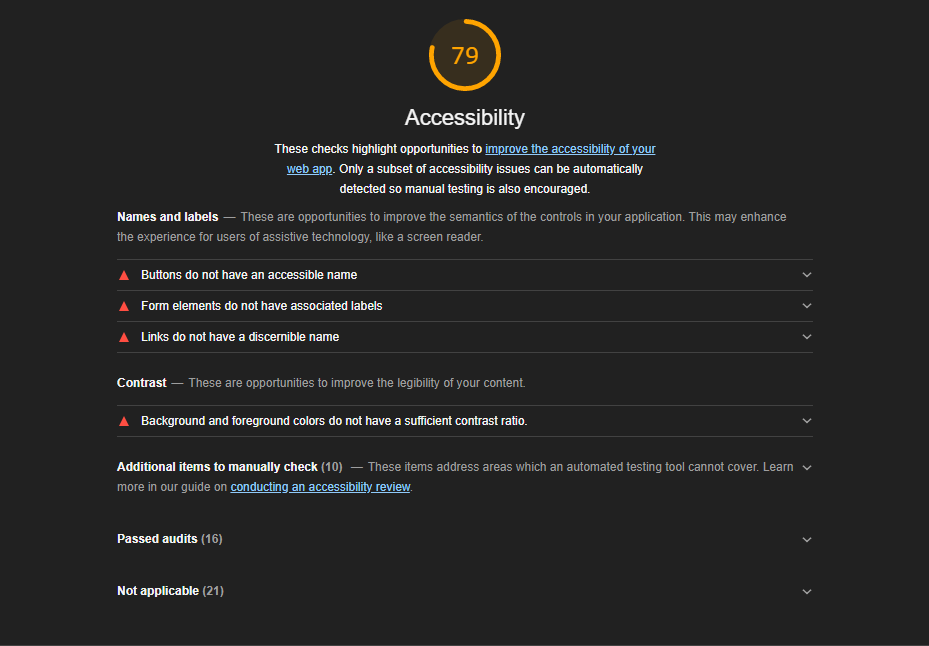
\includegraphics[width=\linewidth]{img/test_accesibilidad}
	\caption[Resultados de las pruebas de accesibilidad]{Resultados de las pruebas de accesibilidad en la mayoría de las vistas de menú}
	\label{fig:testaccesibilidad}
\end{figure}

Además, aunque de menor importancia, se han detectado anomalías en cuanto al poco contraste entre el fondo y el contenido, de manera que las personas con una visión reducida podrían tener problemas al visualizar la web. Podríamos, en este caso, ofrecer una visualización alternativa en cuanto al esquema de colores respecta, ya que no sería muy complicado aplicar unas cuantas reglas adicionales y que se ejecutaran de forma opcional para las personas con este tipo de necesidades.

Sobre la lacra de etiquetas en los campos de un formulario que detecta Lighthouse \cite{lighthouse}, es en este caso en el lado de la clase que renderiza los campos de búsqueda de la tabla del menú, que probablemente puedan configurarse de alguna manera, solo que al ser generados de forma automática, no se les ha prestado gran atención a los mismos.

\section{Credenciales para la prueba en primera personad de twinX}

Para poder experimentar el funcionamiento de twinX (accesible en \cite{twinx}) y ejecutar una serie de pruebas, se pone a disposición del lector las siguientes credenciales:

\begin{itemize}
	\item Entorno de \gls{gestortwinX}:
	\begin{itemize}
		\item \textbf{Nombre de usuario:} gestor
		\item \textbf{Contrseña:} gestor	
	\end{itemize}
	\item Entorno de \gls{administradortwinX}:
	\begin{itemize}
		\item \textbf{Nombre de usuario:} administrador
		\item \textbf{\textsc{Contraseña}:} administrador	
	\end{itemize}
\end{itemize}


